\begin{figure}
  \centering
  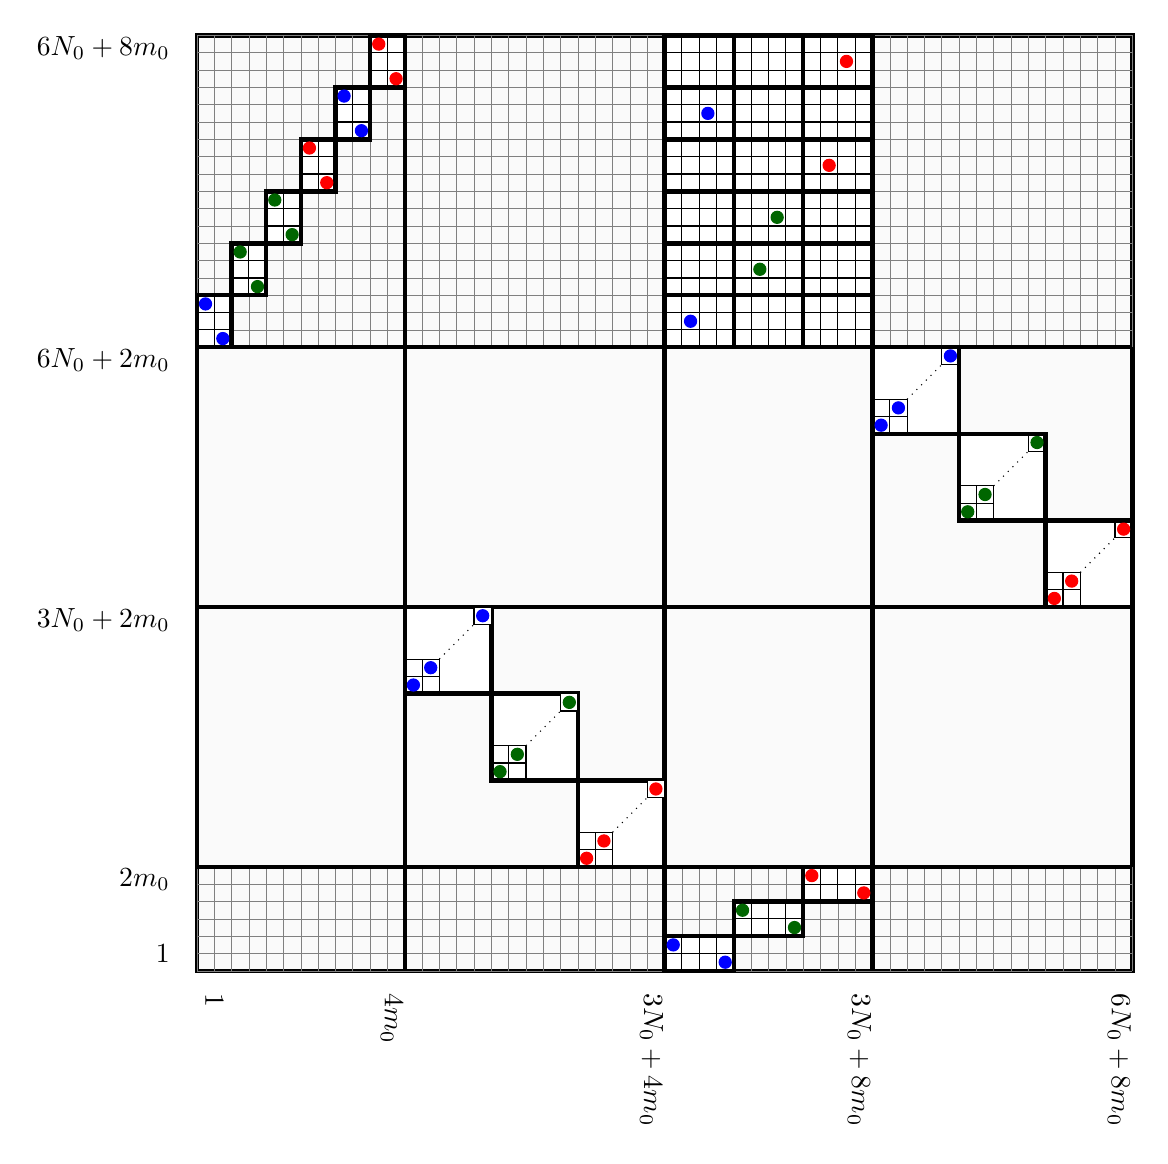
\begin{tikzpicture}
    [
      scale=.22,
    ]
    % 0-areas
    % \draw [fill=black!5] (0,0) rectangle (12,6);
    % \draw [fill=black!5] (0,6) rectangle (12,21);
    % \draw [fill=black!5] (0,21) rectangle (12,36);
    % \draw [fill=black!5] (2,36) -- (12,36) -- (12,51) -- (10,51) -- (10,48) -- 
    %                                (8,48)  --  (8,45) -- (6,45)  -- (6,42)  -- 
    %                                (4,42)  --  (4,39) -- (2,39)  -- (2,)  -- cycle;

    % grid
    \draw [black, ultra thick,fill=black!2] (0,0) rectangle (54,54);
    \draw [step=1.0, help lines] (0,36) grid (54,54);
    \draw [step=1.0, help lines] (0,0) grid (54,6);
    \draw [black, ultra thick] (12,0) -- (12,54);
    \draw [black, ultra thick] (27,0) -- (27,54);
    \draw [black, ultra thick] (39,0) -- (39,54);
    \draw [black, ultra thick] (0,6) -- (54,6);
    \draw [black, ultra thick] (0,21) -- (54,21);
    \draw [black, ultra thick] (0,36) -- (54,36);

    % x-labels
    \node [rotate=-90,anchor=west] at (1, -.75)  {$1$};
    \node [rotate=-90,anchor=west] at (12 - .75, -.75) {$4m_0$};
    \node [rotate=-90,anchor=west] at (27 - .75, -.75) {$3N_0 + 4m_0$};
    \node [rotate=-90,anchor=west] at (39 - .75, -.75) {$3N_0 + 8m_0$};
    \node [rotate=-90,anchor=west] at (54 - .75, -.75) {$6N_0 + 8m_0$};

    % y-labels
    \node [anchor=east] at (-1, 1) {$1$};
    \node [anchor=east] at (-1, 6 - .75) {$2m_0$};
    \node [anchor=east] at (-1, 21 - .75) {$3N_0 + 2m_0$};
    \node [anchor=east] at (-1, 36 - .75) {$6N_0 + 2m_0$};
    \node [anchor=east] at (-1, 54 - .75) {$6N_0 + 8m_0$};

    % vertices
    \def\y{36}
    \foreach \i/\c in {1/blue,2/black!60!green,3/black!60!green,4/red,5/blue,6/red} {
      \draw [black, fill=white, ultra thick] (2*\i - 2, \y + 3*\i - 3) rectangle (2*\i, \y + 3*\i);
      \draw [step=1.0, black] (2*\i - 2, \y + 3*\i - 3) grid (2*\i, \y + 3*\i);
      \draw [\c,fill=\c] (2*\i - 1.5, \y + 3*\i - .5) circle (0.35);
      \draw [\c,fill=\c] (2*\i - .5, \y - 2 + 3*\i - .5) circle (0.35);
    }
    
    % edges
    \draw [black, fill=white] (27,36) rectangle (39, 54);
    \draw [step=1.0, black] (27,36) grid (39, 54);
    \draw [black, ultra thick] (27,36) rectangle (39, 54);
    \foreach \k/\i/\j/\c in {1/1/5/blue,2/2/3/black!60!green,3/4/6/red} {
      \draw [black, fill=white,ultra thick] (4*\k + 23, 2*\k - 2) rectangle (4*\k + 27, 2*\k);
      \draw [step=1.0, black] (4*\k + 23, 2*\k - 2) grid (4*\k + 27, 2*\k);
      \draw [\c,fill=\c] (4*\k + 23 + 1 - .5, 2*\k - .5) circle (0.35);
      \draw [\c,fill=\c] (4*\k + 23 + 4 - .5, 2*\k - 1 - .5) circle (0.35);
      \draw [\c,fill=\c] (4*\k + 23 + 2 - .5, 36 + 3*\i - 1 - .5) circle (0.35);
      \draw [\c,fill=\c] (4*\k + 23 + 3 - .5, 36 + 3*\j - 1 - .5) circle (0.35);
    }
    % horizontal
    \draw [black, ultra thick] (31, 36) -- (31, 54);
    \draw [black, ultra thick] (35, 36) -- (35, 54);
    % vertical
    \draw [black, ultra thick] (27, 39) -- (39, 39);
    \draw [black, ultra thick] (27, 42) -- (39, 42);
    \draw [black, ultra thick] (27, 45) -- (39, 45);
    \draw [black, ultra thick] (27, 48) -- (39, 48);
    \draw [black, ultra thick] (27, 51) -- (39, 51);


    % separators 2
    \def\x{39}
    \def\y{31}
    \foreach \i/\c in {1/blue,2/black!60!green,3/red} {
      \def\xs2{\x + 5*\i - 5}
      \def\ys2{\y - 5*\i + 5}
      \draw [black, fill=white, ultra thick] (\xs2, \ys2) rectangle (\xs2 + 5, \ys2 + 5);
      \draw [step=1.0, black] (\xs2, \ys2) grid (\xs2 + 2, \ys2 + 2);
      \draw [dotted] (\xs2 + 2, \ys2 + 2) -- (\xs2 + 4, \ys2 + 4);
      \draw [black] (\xs2 + 4, \ys2 + 4) rectangle (\xs2 + 5, \ys2 + 5);
      \draw [\c,fill=\c] (\xs2 + .5, \ys2 + .5) circle (0.35);
      \draw [\c,fill=\c] (\xs2 + 1.5, \ys2 + 1.5) circle (0.35);
      \draw [\c,fill=\c] (\xs2 + 4.5, \ys2 + 4.5) circle (0.35);
    }

    % separators 1
    \def\x{12}
    \def\y{16}
    \foreach \i/\c in {1/blue,2/black!60!green,3/red} {
      \def\xs2{\x + 5*\i - 5}
      \def\ys2{\y - 5*\i + 5}
      \draw [black, fill=white, ultra thick] (\xs2, \ys2) rectangle (\xs2 + 5, \ys2 + 5);
      \draw [step=1.0, black] (\xs2, \ys2) grid (\xs2 + 2, \ys2 + 2);
      \draw [dotted] (\xs2 + 2, \ys2 + 2) -- (\xs2 + 4, \ys2 + 4);
      \draw [black, fill=white] (\xs2 + 4, \ys2 + 4) rectangle (\xs2 + 5, \ys2 + 5);
      \draw [\c,fill=\c] (\xs2 + .5, \ys2 + .5) circle (0.35);
      \draw [\c,fill=\c] (\xs2 + 1.5, \ys2 + 1.5) circle (0.35);
      \draw [\c,fill=\c] (\xs2 + 4.5, \ys2 + 4.5) circle (0.35);
    }
  \end{tikzpicture}
  \caption{\label{fig:example-merge-permutation-pi0}
    Transforming the matching \raisebox{-.25cm}{\EXAMPLEM} into the permutation $\pi^0$.
    In this example, each separator is an increasing pattern of length $N_0 = 8 \times 3 + 1 = 25$.
  }% end caption
\end{figure}